\chapter{Project planning}
Project planning is very necessary on the IT and Data Science world. Decades ago many projects failed due to the lack of organization, so it's important to use some framework to divide the project in different task and set deadlines.

An appropriate planning ensures that goals are met in due time, assigning the adequate resources and minimizing risks. As Data Science operates in the intersection between Computer Science, Maths and subject expertise, we will apply a Software Engineering development methodology.
They can be classified in two big groups \cite{traditional-vs-agile}:
\begin{itemize}
    \item Traditional: Based on pre-organized phases in which the flow of development is unidirectional. They are adequate for projects with very clear requisites, like the ones in construction, where the client exactly knows what he wants so there won't be major changes in the future.
    \item Agile: They can share the same phases as the traditional ones, but they are applied in an incremental and cyclic fashion. At the end of each cycle, a prototype is delivered to the client so he can review it and propose changes: these kind of methodologies are great for fast-paced industries where requirements change and the final product specifications are not completely clear. This is the case of current software development market.
\end{itemize}
By the nature of this project the author has decided to apply an agile methodology, handing in different deliverables to the project supervisor during its development. Concretely, he will use the SCRUM methodology.

\section{SCRUM methodology}
On this type of agile methodology, three phases are found, as can be seen in Figure \ref{fig:scrum-phases} \cite{schwaber1997scrum}.
\begin{enumerate}
    \item Planning phase: Well-defined process where inputs and outputs are clear. On it, the project is defined indicating some initial requisites.
    \item Sprints: Each one of the cycles we talked about in the beginning of this chapter. On it, the project is developed and integrated with previous sprints. Nevertheless, they are non-linear and flexible and there could be differences in their structure between them. Sprints normally take between 2 and 5 weeks and at their end a deliverable can be handed in to the client: when he is satisfied with the result, the final product has been reached.
    \item Closure: Again, a well-defined process in which the final product is prepared to be delivered to the client.
\end{enumerate}
An important person in SCRUM management is the SCRUM Master, who interacts frequently with the development team and the product owner to ensure that the project fulfills the client needs.

\begin{figure}[H]
\centering
    \caption{SCRUM development methodology phases \cite{schwaber1997scrum}.}
    \label{fig:scrum-phases}
    \fbox{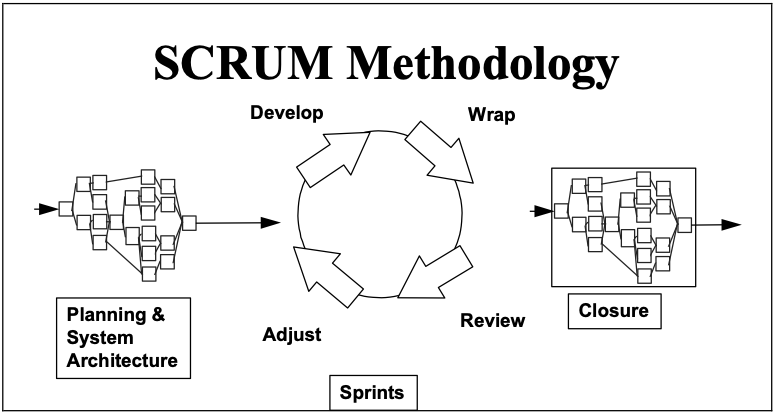
\includegraphics[scale=0.4]{images/planning/scrum_phases}}
\end{figure}

\section{Tasks and scheduling}
To accomplish the project objectives the following tasks are proposed:
\begin{itemize}
    \item \textbf{[T1]} Study of the state of the art of the problem.
    \begin{itemize}
        \item \textbf{[T1.1]} Study of the Spanish electrical market, understanding the agents, processes and variables that conform it.
        \item \textbf{[T1.2]} Review of the literature about time series analysis and forecasting, understanding the different techniques and tools that can be useful to meet our objectives.
    \end{itemize}
    \item \textbf{[T2]} Find the necessary data to perform the study.
    \begin{itemize}
        \item \textbf{[T2.1]} Download the data from the internet, either manually or automatically through an API.
        \item \textbf{[T2.2]} Preprocess and study the downloaded data.
    \end{itemize}
    \item \textbf{[T3]} Perform the analysis over the data.
    \begin{itemize}
        \item \textbf{[T3.1]} Forecast prices in the short, medium and long terms.
        \item \textbf{[T3.2]} Study which variables are affecting the electricity price on the short, medium and long term.
    \end{itemize}
    \item \textbf{[T4]} Document the results in this report.
\end{itemize}

It is important to allocate a reasonable time frame for each task.
This project is framed in a 6 credit Master Thesis which means 150 hours of work, we will split this hours through 9 sprints, of two weeks each. That means 9 hours of work per week approximately. The initial scheduling is exposed in the Gantt diagram in Figure \ref{fig:planning-gantt}.

\begin{figure}[H]
\centering
    \caption{Gantt diagram with project task scheduling.}
    \label{fig:planning-gantt}
    \fbox{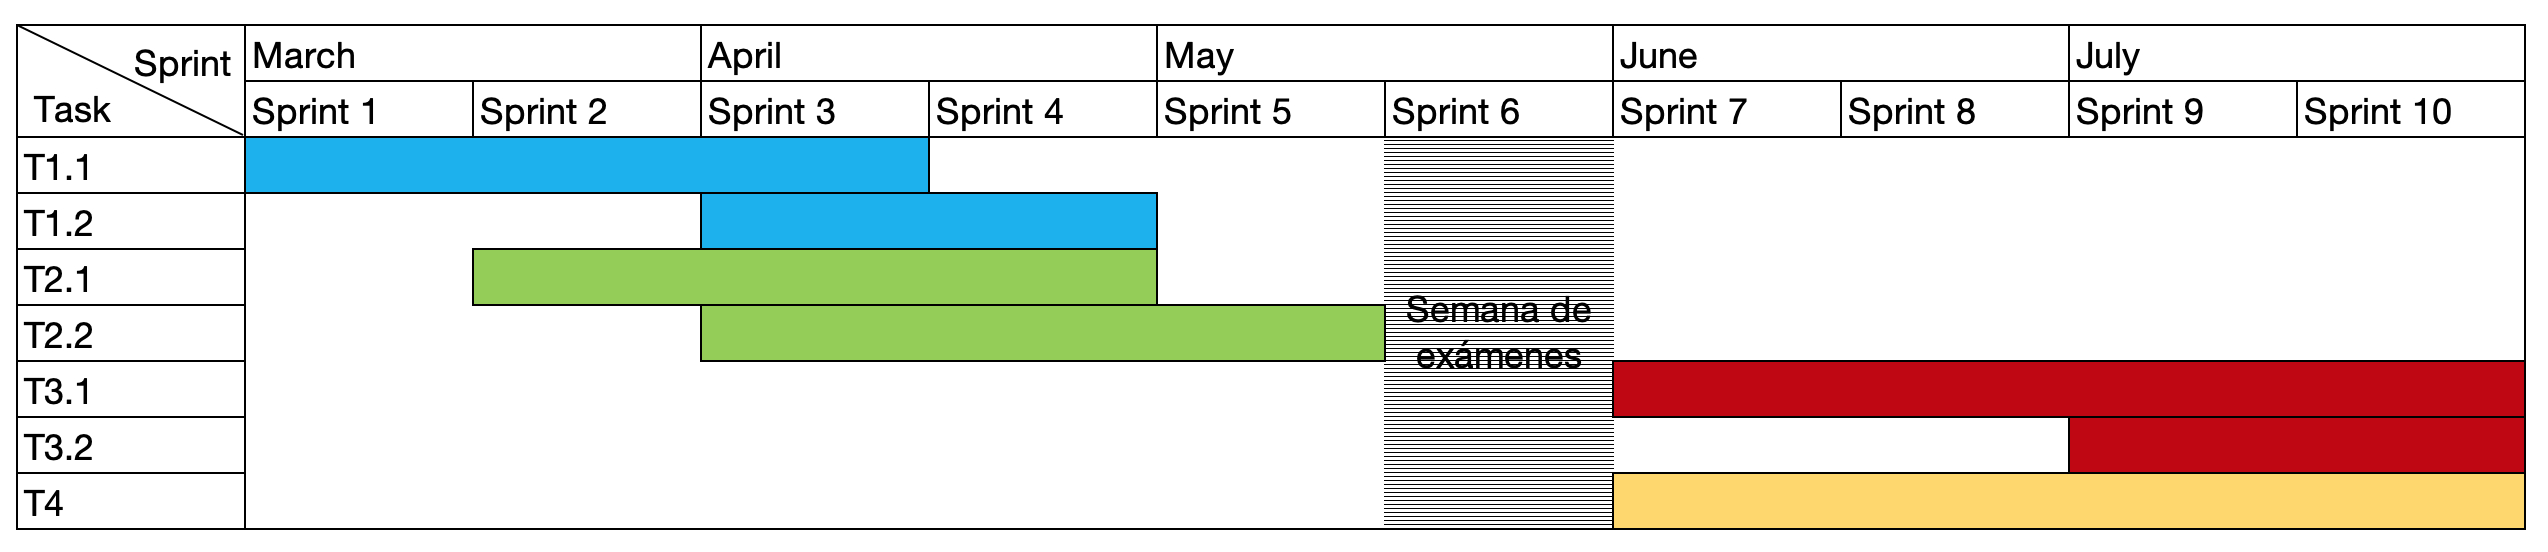
\includegraphics[scale=0.33]{images/planning/planning_gantt}}
\end{figure}